\documentclass{article}

% Use the following line for the initial blind version submitted for review:
\usepackage{icml2020}

% If accepted, instead use the following line for the camera-ready submission:
%\usepackage[accepted]{icml2020}
\usepackage{xr}
\externaldocument{supplementary.tex}
\usepackage{natbib}

\usepackage[utf8]{inputenc} % allow utf-8 input
\usepackage[T1]{fontenc}    % use 8-bit T1 fonts
\usepackage{hyperref}       % hyperlinks
% Attempt to make hyperref and algorithmic work together better:
\newcommand{\theHalgorithm}{\arabic{algorithm}}

\usepackage{url}            % simple URL typesetting
\usepackage{booktabs}       % professional-quality tables
\usepackage{amsfonts}       % blackboard math symbols
\usepackage{nicefrac}       % compact symbols for 1/2, etc.
\usepackage{microtype}      % microtypography
\usepackage{multirow}				% for multi-row labels
\usepackage{subfig}					% for laying out multi-panel figures and tables 
\usepackage{cancel}					% for crossing out characters
\usepackage{amsmath}				% for splitting multi-line equations
\usepackage{placeins}				% for table and figure positioning
\usepackage{mathtools}			% for \vdotswithin{}
\usepackage{resizegather}   % for gathering multi-lines to one line
%packages for graph layout
\usepackage{graphicx}
\usepackage[pdf]{graphviz}

%format section headings compactly
\usepackage[compact]{titlesec}
\titlespacing{\section}{0pt}{2ex}{1ex}
\titlespacing{\subsection}{0pt}{1ex}{0ex}
\titlespacing{\subsubsection}{0pt}{0.5ex}{0ex}

\setlength{\textfloatsep}{3pt}

\icmltitlerunning{Identification of Latent Variables From Residuals}

\begin{document}

\twocolumn[
\icmltitle{Identification of Latent Variables From Their
Footprint In Bayesian Network Residuals}

\icmlsetsymbol{equal}{*}

\begin{icmlauthorlist}
\icmlauthor{Boris Hayete}{equal,former}
\icmlauthor{Fred Gruber}{equal,gns}
\icmlauthor{Anna Decker}{former}
\icmlauthor{Raymond Yan}{gns}
\end{icmlauthorlist}

\icmlaffiliation{former}{Work completed at GNS Healthcare, Cambridge, Massachusetts, USA 02142}
\icmlaffiliation{gns}{Department Of Precision Medicine, GNS Healthcare, Cambridge, Massachusetts, USA 02142}

\icmlcorrespondingauthor{Boris Hayete}{boris@borisland.com}
\icmlcorrespondingauthor{Fred Gruber}{fred@gnshealthcare.com}

\icmlkeywords{Machine Learning, ICML, Computational Biology, Bayes Nets, Latent Variables} %revise!!!!!!!!!!!!!!!!!
\vskip 0.1in
]

\printAffiliationsAndNotice{\icmlEqualContribution} % otherwise use the standard text.

% Set sizes of skips before/after equations, figures, and tables
\setlength{\abovedisplayskip}{4pt}
\setlength{\belowdisplayskip}{4pt} 
\setlength{\belowcaptionskip}{-5pt}

\begin{abstract}
Graph-based causal discovery methods aim to capture conditional independencies consistent with the observed data and differentiate causal relationships from indirect or induced ones.  Successful construction of graphical models of data depends on the assumption of causal sufficiency: that is, that all confounding variables are measured. When this assumption is not met, learned graphical structures may become arbitrarily incorrect and effects implied by such models may be wrongly attributed, carry the wrong magnitude, or mis-represent direction of correlation.  Wide application of graphical models to increasingly less curated "big data" highlights the need for continued attention to the unobserved confounder problem.  

We present a novel method that aims to control for the latent structure of the data in the estimation of causal effects by iteratively deriving proxies for the latent space from the entirety of residuals of the inferred graphical model.  When used for gaussian graphical models, under mild assumptions our method improves structural inference and enhances identifiability of the causal effect. In addition, when the model is being used to predict outcomes, this method un-confounds the coefficients on the parents of the outcomes and leads to improved predictive performance when out-of-sample regime is very different from the training data.  We show that such improvement of the predictive model is intrinsically capped and cannot rise beyond a certain limit as compared to the confounded model.  Furthermore, we propose an algorithm for computing a ceiling for the dimensionality of the latent space which may be useful in future approaches to the problem.  We extend our methodology beyond GGMs to ordinal variables and nonlinear cases.  Our R package provides both PCA and autoencoder implementations of the methodology, suitable for GGMs with some guarantees and for better performance in general cases but without such guarantees. 
\end{abstract}

\section{Introduction}
\label{introduction}

Construction of graphical models (GMs) at its heart pursues two related objectives: accurate inference of the structure of conditional independencies and construction of models for outcomes of interest with the purpose of estimating the average causal effect (ACE) with respect to interventions (\cite{pearl_causality:_2000}, \cite{hernan_estimating_2006}).  These two distinct goals mandate that certain identifiability conditions for both types of tasks be met.  Of particular interest to this work is the condition of \textit{causal sufficiency} (\cite{spirtes_causation_1993}) - namely, whether all of the relevant confounders have been observed.  When this condition is not met, accurate GMs and identifiability of the causal effects are hard to infer.


Intuitively, the presence of unobserved confounding leads to violations of conditional independence among the affected variables downstream from any latent confounder.  Likelihood methods for GM construction aim to minimize unexplained variance for all variables in the network by accounting for conditional independencies in the data (\cite{pearl_causality:_2000}, \cite{friedman_being_2013}).  Lack of observability of a causally important variable will induce dependencies among its descendants in the graph that cannot be fully ascribed to any single child node of the latent variable except by chance due to noise.  Such unexplained interdependency results in model residuals that are correlated with the latent variable and not fully explained by any putative graph parents. Thus, we observe inferred connectivity that is excessive compared to the true network.  (\cite{elidan_discovering_2001}).  


Hitherto, the literature has largely focused on addressing the subset of problems where the ACE can be estimated reliably in the absence of this guarantee, such as when conditional exchangeability holds \cite{hernan_estimating_2006}.  Previously, methods have been proposed for inferring latent variables affecting GMs by the means of expectation maximization (EM) (as far back as \cite{friedman1997learning}, \cite{friedman1998bayesian}).  However, for a large enough network, local gradients do not provide a reliable guide, nor do they address the cardinality of the latent space.  Methods for using near-cliques for detection of latent variables in directed acyclic graphs (DAGs) with gaussian graphical models (GGMs) have been proposed that address both problems by analyzing near-cliques in DAGs (\cite{elidan_discovering_2001}, \cite{silva_learning_2006}).  A method related to ours has been proposed for calculating latent variables in a greedy fashion in linear and "invertible continuous" networks, and relating such estimates to observed data to speed up structure search and enable discovery of hidden variables (\cite{elidan_ideal_2007}). However, with a clique-driven approach it is impossible to tell whether any cliques have shared parents and, importantly, whether any signal remained to be modeled, resulting in score-based testing rejecting proposed "ideal parents". Additionally, Wang and Blei (2019) introduced the deconfounder approach to detecting and adjusting for latent confounders of causal effects in the presence of multiple causes but in the context of a fixed DAG under relatively strict conditions \cite{wang_deconfounder_2019}. 

We show that there exist circumstances when causal sufficiency can be asymptotically achieved and exchangeability ensured even when the causal drivers of outcome are confounded by a number of latent variables.  This can be achieved when the confounding is \textbf{pleiotropic}, that is,  when the latent variable affects a "large enough" number of variables, some driving an outcome of interest and others not (\cite{anandkumar_learning_2013}).  Notably, this objective cannot be achieved when confounding affects only the variables of interest and their causal parents (\cite{damour_multi-cause_2019}). We detail an algorithm for diagnosing and accounting for latent confounding in closed form for a GGM example, demonstrate the implementation in a simulated data set, and discuss extensions to other functional forms.  Importantly, our approach uses an indication of latent space that is global, though only locally optimal, being derived from the totality of network residuals. This allows for one-step derivation of the best local approximation of latent space, leading to theiterative algorithm proposed below.

The outline of this paper is as follows: In the first two sections, we outline the process of diagnosting latent confounding in the special case of GGMs where closed-form solutions exist. In the third section, we derive the improvement cap for predictive models improvements to the graph learned from the data. In the fourth section, discuss implementation, and in the fifth demonstrate the approach in simulated [and real] data. Finally, we discuss some extensions to the approach for more complex graphical model structures and functional forms. 

\section{Background And Notation}
\label{Background}

Consider a factorized joint probability distribution over a set of observed and latent variables Table \ref{tab:notation} summarizes the notation to be used to distinguish variables, their relevant partitions , and parameters. 


\begin{table}[h]
\centering
\scalebox{0.85}{
\begin{tabular}{ c|c|c } 
 Set & Meaning & Indexing \\ 
 \hline
 $S$ & samples & $S_i, i \in \{1, \dots, s\}$ \\ 
 $V$ & observed predictor variables & $V_j, j \in \{1, \dots, v\}$ \\
 $U$ & unobserved predictor variables & $U_l, l \in \{1, \dots, u\}$ \\
 $O$ & outcomes (sinks) & $O_k, k \in \{1, \dots, o\}$ \\
 $D$ & $\{V, O\}$ - observable data & \\
 $D_u$ & $\{V, O, U\}$ - implied data & \\
 $\theta$ & parameters & $\theta_i, i \in \{1, \dots, t\}$ \\
 $Pa^N$ & parents of variable $N$ & $Pa^N_i, i \in \{1, \dots, p\}$\\
 $C^N$ & children of variable $N$ & $C^N_i, i \in \{1, \dots, c\}$\\
 $G$ & graph over $D$ &\\
 $G_u$ & graph over $D_u$&
\end{tabular}}
\smallskip
\caption{Notation}
\label{tab:notation}
\end{table}

Assume that the joint distribution $D_{u}$ over the full data or $D$ over the observed data is factorized as a directed acyclic graph, $G_{u}$ or $G$.  We will consider individual conditional probabilities describing nodes and their parents, $P(V | Pa{V}, \theta)$, where $\theta$ refers to the parameters linking  the parents of $V$ to $V$.  $\hat{\theta}$ will refer to an estimate of these parameters.  We will further assume that $G$ is constructed subject to regularization and using unbiased estimators for $P(V | Pa{V}), \hat{\theta}$.  We will further assume that $D_u$ plus any given constraints are sufficient to infer the true graph up to Markov equivalence.  For convenience, we'll focus on the actual true graph's parameters, so that, using unbiased estimators, $E[\hat{\theta_m}|D_u] = \theta_m, \forall m$.

Mirroring $D$ (or $D_u$), we will define a matrix $R$ (or $R_u$) of the same dimensions - $s \times (v + o)$ (or $s \times (v + o + u)$) - that captures the residuals of modeling every variable $N \in \{V, O, (U)\}$ via $G$ (or $G_u$).  In the linear case, these would be regular linear model residuals, but more generally we will consider probability scale residuals (PSR, \cite{shepherd_probability-scale_2016}).  That is, we define $R[i, j] = PSR(P(V_j | parents(V_j), \hat{\theta}_j) | D[i, j])$, the residuals of $V_j$ given its graph parents.  Notice that the use of probability-scale residuals allows us to define $R$ and $R_u$ for all ordinal variable types, up to rank-equivalence.

\section{Diagnosing Latent Confounding} 

Here, we consider the special case of GGMs where our approach for determining the existence latent confounders can be written down in a closed form. 

Recall that, for some $V_j \in \{V, U, O\}$, $P^{V_j}_k$ denotes the $k$th parent of $V_j$.  For GGMs, we can write down a fragment of any DAG G as a linear equation where a child node is parameterized as a linear function of its parents:
\begin{equation}
\begin{align*}
V_j = \beta_{j0} + \beta_{j1} P^{V_j}_1 + \dots + \beta_{jp} P^{V_j}_p + \xi_j,\\\xi_j \sim \mathcal{N}(0, \sigma_j).
\end{align*}
\end{equation}	

\FloatBarrier
\begin{figure}[h]
	\centering
	\begin{minipage}[t]{\dimexpr0.6\textwidth}
	\digraph[scale=0.5]{g}{
			graph[ranksep=0.1];
      node [shape=circle, style="filled"];
      U [fillcolor=red];
      V1 [fillcolor=white, label=<V<SUB>1</SUB>>];
      V2 [fillcolor=gray, label=<V<SUB>2</SUB>>];
      V3 [fillcolor=gray, label=<V<SUB>3</SUB>>];
      V4 [fillcolor=gray, label=<V<SUB>4</SUB>>];
      V5 [fillcolor=gray, label=<V<SUB>5</SUB>>];
      V6 [fillcolor=gray, label=<V<SUB>6</SUB>>];
      V7 [fillcolor=white, label=<V<SUB>7</SUB>>];
      O1 [fillcolor=green, label=<O<SUB>1</SUB>>];
      O2 [fillcolor=green, label=<O<SUB>2</SUB>>];
      V1 -> U; U -> V2; U -> V3; U-> V4; U-> V5; U -> V6; V1 -> O2; V2 -> O2; V4-> O1; V5 -> O1; V6 -> O1; U -> O2; U -> O1; V1 -> V2; V5 -> V6; V7 -> O1
	}
	\begin{minipage}{\dimexpr0.8\textwidth}
	\caption{Graph $G_u$.  $U$ influences the outcomes $O$, and a number of predictors $V$, confounding many of the $V_j \rightarrow O_k$ relationships.  Gray nodes are affected by $U$.}
	\label{fig:sampleGraph}
	\end{minipage}
	\end{minipage}\hfill
	\begin{minipage}[t]{\dimexpr0.6\textwidth}
	\digraph[scale=0.5]{g2}{
			graph[ranksep=0.1];
      node [shape=circle, style="filled"];
      V1 [fillcolor=white, label=<V<SUB>1</SUB>>];
      V2 [fillcolor=gray, label=<V<SUB>2</SUB>>];
      V3 [fillcolor=gray, label=<V<SUB>3</SUB>>];
      V4 [fillcolor=gray, label=<V<SUB>4</SUB>>];
      V5 [fillcolor=gray, label=<V<SUB>5</SUB>>];
      V6 [fillcolor=gray, label=<V<SUB>6</SUB>>];
      V7 [fillcolor=white, label=<V<SUB>7</SUB>>];
      O1 [fillcolor=green, label=<O<SUB>1</SUB>>];
      O2 [fillcolor=green, label=<O<SUB>2</SUB>>];
      V1 -> V3; V3 -> V2; V3 -> V4; V3 -> V6; V3 -> V5; V4 -> V6; V6 -> V5; V1 -> O2; V2 -> O2; V4-> O1; V5 -> O1; V6 -> O1; V7 -> O1; V3 -> O2; V4 -> V5; V5 -> O2; V1 -> V2; V2 -> V5; V3 -> O1
	}
	\begin{minipage}{\dimexpr0.8\textwidth}
	\caption{Graph $G$.  With $U$ latent, the graph adjusts, introducing spurious edges.}
	\label{fig:sampleGraphOnObservables}
	\end{minipage}
	\end{minipage}
\end{figure}
\FloatBarrier

For example, consider $O_1$ in Figure \ref{fig:sampleGraph}.  We can write:
\begin{equation}
\begin{split}
O_1 = \beta_0 + \beta_6V_6 + \beta_5V_5 + \beta_4V_4 + \beta_7V_7 + \beta_uU + \xi_1,\\ \xi_1 \sim \mathcal{N}(0, \sigma_{O_1}).
\end{split}
\end{equation}

For any variable N that has parents in $G_u$, we can group variables in $P^N$ into three subsets: $X_U \in \{P^U, C^U\}$, $X_{\cancel{U}} \notin \{P^U, C^U\}$, and the set $U$ itself, and write down the following general form using matrix notation:
\begin{equation}
\begin{split}
N = \beta_{N0} + B_U X_U + B_{\cancel{U}} X_{\cancel{U}} + \beta_U U + \xi_N,\\\xi_N \sim \mathcal{N}(0, \sigma_{N}).
\end{split}
\label{eq:linearForm}
\end{equation}

Explicit dependence of $N$ on $U$ happens when $\beta_U \neq 0$.  

Now consider $G$,  the graph built over the variables $\{V, O\}$ excluding the latent space $U$.  Note that if we deleted $U$ and its edges from $G_u$ without rebuilding the graph, Equation \ref{eq:linearForm} from $G_u$ would read:
\begin{equation}
N = \beta_{N0} + B_U X_U + B_{\cancel{U}} X_{\cancel{U}} + R_N + \xi_N. 
\label{eq:linearFormNoU}
\end{equation}
The residual term $R_N$ is simply equal to the direct contribution of $U$ to $N$.  The network $G$ would have to adjust to the missingness of $U$ (e.g., Figure \ref{fig:sampleGraphOnObservables} vs Figure \ref{fig:sampleGraph}).  As a result, $R_N$ will be partially substituted by other variables in $\{P^U, C^U\}$.  Still, unless $U$ is completely explained by $\{P^U, C^U\}$ (as described in \cite{damour_multi-cause_2019}) and in the absence of regularization (when a high enough number of covariates may lead to such collinearity), $R_N$ will not fully disappear in $G$.  Hence, even after partially explaining the contribution of $U$ to $N$ by some of the parents of $N$ in $G$, 
\begin{equation}
R_N = \beta_0 + \beta_1 U + \xi_N.
\label{eq:residualColumn}
\end{equation}

\begin{center}
\begin{table}[ht]
\centering
\scalebox{1}{
\begin{tabular}{c|c|c|c|c|}
&\multicolumn{4}{c}{Variables}\\
\hline
\multirow{3}{*}{\rotatebox[origin=c]{90}{Samples  }}
&$V_{11}$&$V_{12}$&\dots&$V_{1v}$\\
&\vdots&\vdots&\vdots&\vdots\\
&$V_{s1}$&$V_{s2}$&\dots&$V_{sv}$\\
\end{tabular}}
\qquad
\qquad
\qquad
\qquad
\scalebox{1}{
\begin{tabular}{c|c|c|c|c|}
&\multicolumn{4}{c}{Residuals}\\
\hline
\multirow{3}{*}{\rotatebox[origin=c]{90}{Samples  }}
&$R_{11}$&$R_{12}$&\dots&$R_{1v}$\\
&\vdots&\vdots&\vdots&\vdots\\
&$R_{s1}$&$R_{s2}$&\dots&$R_{sv}$\\
\end{tabular}}
\caption{The training data frame (Variables) implies a matching data frame (Residuals) once the joint distribution of all variables is specified via a graph and its parameterization}
\label{tab:MatchingResiduals}
\end{table}
\end{center}

Therefore, the columns in the residuals table corresponding to $G$ (Table \ref{tab:MatchingResiduals}) that represent the parents and children of $U$ will contain residuals collinear with $U$:
\begin{equation}
\begin{split}
R_1 = \beta_{10} &+ \beta_{11} U + \xi_1\\
& \vdots\\
R_k = \beta_{k0} &+ \beta_{k1} U + \xi_k.
\end{split}
\end{equation}

Rearranging and combining,
\begin{equation}
U = \beta_i^{*} R_1 + \dots + \beta_k^{*} R_k + \xi = B R + \xi.
\label{eq:resPCA}
\end{equation}

Equation \ref{eq:resPCA} tells us that, for graphical gaussian models, components of $U$ are obtainable from linear combinations of residuals, or principal components (PCs) of the residual table $R$.  In other words, $U$ is identifiable by principal component analysis (PCA).  Whether the residuals needed for this identification exist depends on the \textit{expansion property} as defined in \cite{anandkumar_learning_2013}.

Note that this approach is similar, in the linear case, to that in \cite{elidan_ideal_2007} except insofar as we show the global principal components of the residual matrix to be optimal for the discovery of the whole latent space of a given DAG assuming its structure is already correct, and we therefore couple structure inference and latent space discovery via EM as separate rather than interleaved steps (\ref{alg:latentEM}).

\section{Capping improvement}

The most important utility of causal modeling is to identify drivers as well as drivers of drivers of outcomes of interest.  These drivers of drivers may have practical importance. For example, in the development of a drug, direct predictors of an outcome (e.g. $V_6$ pointing to $O_{1}$ in Figure \ref{fig:sampleGraph}) may not be viable targets but upstream variables (e.g. $V_{5}$) may in fact be be promising targets and the direct parents of the outcome mediate the effect of these potential targets. In the presence of latent confounding, the identifiability of causal effects of outcomes is jeopardized \cite{hernan_estimating_2006}.  For example, in Figure \ref{fig:sampleGraph} $U$ induces correlation among $V_3$, $V_4$, $V_5$, and $V_6$ even when these variables are conditionally independent given $U$.  

The extent of the problem of unmeasured confounding can be quantified in more detail.  Suppose we model $O_1$ without controlling for $U$ (\ref{fig:sampleGraphOnObservables}): $$O_1 = \beta_0 + \beta_3 V_3 + \beta_4 V_4 + \beta_5 V_5 + \beta_6 V_6 + \dots.$$  Setting the coefficient of determination for the model $$V_3 = \alpha_0 + \alpha_4 V_4 + \alpha_5 V_5 + \alpha_6 V_6 + \dots.$$ equal to $\rho_3^2$.  Then the estimated variance of $\beta_3$ in the presence of collinearity can be related to the variance when collinearity is absent via the following formula (\cite{rawlings_applied_1998}):
\begin{equation}
var(\bar{\beta}_3) = var(\beta_3) \frac{1}{1-\rho_3^2} \propto \frac{1}{1-\rho_3^2}.
\label{eq:VIF}
\end{equation}
Formula \ref{eq:VIF} describes the \textit{variance inflation factor} (VIF) of $\beta_3$.  Note that $\lim_{\rho \to 1} \frac{1}{1-\rho^2} = \infty$, so even mild collinearity induced by latent variables can severely distort coefficient values and signs, and thus estimation of ACE.  Our approach reduces the VIFs of coefficients related to outcomes and thus make all \textit{causal} statements relating to outcomes, such as calculation of ACE, more reliable, by controlling for $\bar{U}$ - the estimate of $U$ - in the network,
\begin{equation}
\lim_{(U - \bar{U})\to0} var(\bar{\beta}_i) = var(\beta_i).
\label{eq:vifImprovement}
\end{equation}

Consider an output $O_j$.  While it is difficult to describe the limit of error on the coefficients of the drivers of $O_j$, it is straightforward to put a ceiling on the improvement in the likelihood obtainable from modeling $U$ and approximating $G_u$ with $G_{\bar{u}}$.  Suppose we eventually model $U$ as a linear combination of a set of variables $X \subset V$, and denote by $X \setminus W$ the set difference: members of $X$ not in $W$.  Then for any outcome $O_i$ predicted by a set of variables $W$ in the graph $G$ and in truth predicted by the set $Z + U$, we can contrast three expressions (from $G$ and $G_{\bar{U}}$ respectively):
\begin{equation}
\begin{split}
O_i = \beta_{i0} + B_W W (a) + \xi_i \qquad (a)\\
O_i = \beta_{i0} + B_W W + B_{X \setminus W} (X \setminus W)
 + \xi_i \qquad (b)\\
O_i^U = \beta_{i0}^U + B_Z^U Z + B^U U + \xi_i \qquad (c).
\end{split}
\end{equation}
Model (a) is the model that was actually accepted, subject to regularization, in G.  Model (b) is the "complete" model of $O_i$ that controls for $U$ non-parsimoniously by controlling for all variables affected by $U$ and not originally in the model.  The third model, (c), is the ideal parsimonious model when U is known.  We can compare the quality of these models via the Bayesian Score, and the full score, which can approximated by the Bayesian Information Criterion (BIC) in large samples (\cite{koller_probabilistic_2009}).  We assume that model (c) would have the lowest BIC (being the best model), and model (a) would be slightly better, since we know that the set of variables $X \setminus W$ didn't make it into the first equation subject to regularization by BIC.  Assuming $n$ samples,

\begin{align}
b_{a} &= BIC(O_{i} = \beta_{i0} + B_W W + \xi_i)  \\
b_{b} &= BIC(O_i = \beta_{i0} + B_W W  \\
               &  + B_{X \setminus W} (X \setminus W) + \xi_i) \nonumber \\
&  = b_c + |X\setminus W| log(n) \nonumber \\
b_{c} &= BIC(O_i^U = \beta_{i0}^U + B_Z^U Z + B^U U + \xi_i)
\end{align}

The "complete model" - model (b) - includes all of the true predictors of $O_j$.  Therefore its score will be the same as that of the true model - model (c) - plus the BIC penalty, $log(n)$, for each extra term, minus the cost of having $U$ in the true model (that is, the cardinality of the relevant part of the latent space).  We know that the extra information carried by this model was not big enough to improve upon model (a), that is $b_a < b_c + k \log(n)$ for some $k$.  Rearranging:
\begin{equation}
    b_c - b_a > -k\log(n).
    \label{eq:ceilingTheorem}
\end{equation}
Any improvement in $G_{\bar{U}}$ owing to modeling of $\bar{U}$ cannot, therefore, exceed $k\log(n)$ logs, where $k = |X \setminus W| - |U|$: the information contained in the "complete" model is smaller than its cost.

Although the available improvement in predictive power is also capped in some way, it is still important to aim for that limit.  The reason is, correct inference of causality, especially in the presence of latent variables, is the only way to ensure transportability of models in real-world (heterogeneous-data) applications (see, e.g., \cite{bareinboim_causal_2016}).

This approach is a generalization of work presented in \cite{anandkumar_learning_2013}, where the authors show that, under some assumptions. the latent space can be learned exactly, which is also related to the deconfounder approach described by \cite{wang_deconfounder_2019}.  However, our approach does not require that the observables be conditionally independent given the latent space and instead \textit{generate} such independence by the use of causal network's residuals, which are conditionally independent of each other \textit{given the graph and the latent space}.  However, since the network among the observables is undefined in the beginning, the structure of the observable network must be learned at the same time as the structure of the latent space, which leads us to the iterative/variational bayes approach presented in Algorithm \ref{alg:latentEM}.  Lastly, the use of the entirety of the residual space is different from the work described in \cite{elidan_ideal_2007}, where local residuals are pursued with the goal to accelerate structure learning while simultaneously discovering the latent space.

\section{Implementation}
Algorithm \ref{alg:latentEM} below describes our approach to learning the latent space and can be viewed as a type of an expectation-maximization algorithm, possibly nested, if EM is used to learn the DAG at each step.

How do we learn $\bar{U} = f(R_{\bar{U}})$?  In the linear case, we can use PCA, as described above, and in the non-linear case, we can use non-linear PCA, autoencoders, or other methods, as alluded to above.  However, the linear case provides a useful constraint on dimensionality, and this constraint can be derived quickly.  A useful notion of the ceiling constraint on the linear latent space dimensionality can be found in \cite{gavish_optimal_2014}.  From a practical standpoint, the dimensionality can be even tighter, and we propose a permutation-test-based method for inferring $ceiling(|U|)$ in Algorithm \ref{alg:linearPCA}.

The integral should converge faster than the count of times variance explained by $U^{*}$ on true residuals exceeds that obtained from shuffled residuals, but the permutation test approach of PCA cardinality is also workable, albeit with more iterations.  Note that it is necessary to correct for the number of tests performed, and that we use Bonferroni correction as a simple and conservative stand-in. Alternatively, networks built using structural priors of the form proposed in \cite{friedman_being_2013} may not need to perform this step.

Our algorithm \ref{alg:linearPCA} is different from that proposed in \cite{elidan_learning_2005}.  If we consider $Y = f(X)$, where $Y$ are all DAG outputs and $X$ are all inputs, and $f$ is a suitably parameterized DAG, PCA over residuals (linear or not) normalized by PCA over shuffled residuals provides a measure of "compressibility" of residual space.  In other words, we propose a minimum description length algorithm for detecting the latent variables so that the residual space is no longer compressible.

%\FloatBarrier
%\begin{center}
%\scalebox{0.5}{
%\begin{minipage}[t]{0.9\textwidth}
\begin{algorithm}%[H]
 \caption{Learning $\bar{U}$ from structure residuals via EM}
 \label{alg:latentEM}
\begin{algorithmic}
%\DontPrintSemicolon
%\SetAlgoLined
 \STATE foobar
 \STATE \textbf{Data:} The set of observed variables $\{V, O\}$
 \STATE \textbf{Result:} Graph $G_{\bar{U}}(V, O, \bar{U})$
 \STATE Construct $G = G(V, O)$\;
 \STATE Compute $S_0 = BIC_{G}$\;
 \STATE Estimate $\bar{U} = f(R)$\;
 \STATE Construct $G_{\bar{U}} = G(V, O, \bar{U})$\;
 \STATE Compute $S_{\bar{U}} = BIC(G_{\bar{U}})$\;
 \WHILE{$S_{\bar{U}} - S_0 > \epsilon$} 
  \STATE Set $S_0 = S_{\bar{U}}$\;
  \STATE Calculate $R_{\bar{U}}$:\;
  \STATE Set $\bar{U}$ to arbitrary constant values\;
  \FORALL{child node $C \in G_{\bar{U}}, C \notin \bar{U}$}
  	\STATE Set parents to training data\;
  	\STATE $\bar{C} = C|parents(C)$\;
  	\STATE Set $R_C = PSR(\bar{C}, C)$\;
  \ENDFOR
  \STATE Estimate $\bar{U} = f(R_{\bar{U}})$\;
  \STATE Construct $G_{\bar{U}} = G(V, O, \bar{U})$\;
  \STATE Compute $S_{\bar{U}} = BIC(G_{\bar{U}})$\;
 \ENDWHILE
\end{algorithmic}
\end{algorithm}
%\end{minipage}
\hspace{1cm}
%\begin{minipage}[t]{1\textwidth}
\begin{algorithm}%[H]
 \caption{Inferring linearly optimal $\bar{U}$ and assessing its cardinality by permutations}
 \label{alg:linearPCA}
\begin{algorithmic}
\STATE {\bfseries Data:} The set of residuals $R_{\bar{U}}$ from modeling $D$ with $G_{\bar{U}}$
\STATE \textbf{Result:} Linear approximation to $\bar{U}$
 \STATE Set significance threshold $\alpha$ (e.g. $\alpha = 0.05$)\;
 \STATE Learn $\bar{U} = PCA(R_{\bar{U}})$\;
 \STATE Calculate column-wise variance explained $V_E^{0}$ for $\bar{U}^{*}$\;
 \STATE Set $V_E^s = 0 \times rank(R_{\bar{U}})$, matrix of variances explained by shuffling\;
 \WHILE{$se(\bar{U}) > \epsilon$} 
  \STATE $R_{\bar{U}}^{*} = shuffle(R_{\bar{U}})$ (column-wise)\;
  \STATE Calculate $\bar{U}^{*} = PCA(R_{\bar{U}}^{*})$\;
  \STATE Calculate $V_E^{*}$ for $\bar{U}^{*}$\;
  \STATE Concatenate row-wise: $V_E^s = \{V_E^s; V_E^{*}\}$\;
  \STATE Fit $B(i)$ beta distributions to each column $i$ of $V_E$\;
  \STATE For each column $i$ of $\bar{U}$, calculate:\;
  \begin{gather*}
  P(V_E^{0}(i) | V_E^s(i)) = \lim_{|V_E^s(i)| \to \infty} \frac{|V_E^s(i) > V_E^{0}(i)|}{|V_E^s(i)|} \approx 1 - \int_{-\infty}^{V_E^{0}(i)} PDF(B_i)
  \end{gather*}\;
 \ENDWHILE
 \STATE $P(V_E^{0}(i) | V_E^s(i)) = P(V_E^{0}(i) \sim V_E^s(i)) \times rank(V_E)$\;
 \STATE Drop $V_E^{0}(i)$ for which $P(V_E^{0}(i) \sim V_E^s(i)) > \alpha$
\end{algorithmic}
\end{algorithm}
%\end{minipage}
%}
%\end{center}
%\FloatBarrier



\subsection{Nonlinear Extension: Autoencoder}

All results described above refer to gaussian or at most rank-monotonic relationships, and perhaps extend to linear models with interactions, when interactions can be seen as "synthetic features". Real-world data, however, often does not behave this way requiring an approach that might generalize beyond monotonic relationships.  Therefore, we pursued latent space discovery using autoencoders.

We first assess the cardinality of the latent space (number of nodes in the coding layer) using the linear approach (PCA), and take this number as a useful "ceiling" for the dimensionality of the non-linear latent space, on the assumption that non-linear features are more compact and require lower dimensionality if discovered.  We then constructed an autoencoder with 4 hidden layers where the maximum number of nodes in the hidden layers was capped at $\min (100, \textrm{number of variables})$, the cap being dictated by practical considerations.

The autoencoder was implemented using Keras with Tensorflow backend and called within R using the Reticulate package \cite{reticulate_2020}. The encoders and decoder were kept symmetric and in order improve the stability we used tied weights (\cite{pca_ae}). In addition, the coding layer had additional properties borrowed from PCA including a kernel regularizer promoting orthogonality between weights and an activity regularizer to promote uncorrelated encoded features (see \cite{ranjan_build_2019} for details on implementation and justification). This last property is of particular interest in our application since ideally every dimension in our latent space should be associated with a different latent variable. The hidden layers used a sigmoidal activation except for the output layer which had a linear activation. All layers had batch normalization \cite{ioffe2015batch} (see supplementary Figure 1 for a diagram of the architecture).

For more details see the implementation in the github repository for this paper (\cite{latent_2020}).

\section{Numerical Demonstration}
\subsection{Synthetic Data}
To illustrate  the algorithms described in the previous sections we
generated synthetic data from the network shown in Figure
\ref{fig_truenet} (also supplementary Figure 2) where two variables $V_1$ and $V_2$ drive an outcome
$Z$. Two confounders $U_1$ and $U_2$ affect both the drivers and the
outcome, as well as many additional variables that do not affect the
outcome $Z$.
The coefficient values in the network were chosen so that faithfullness (also knows as stability \cite{pearl_causality:_2000}) was achieved allowing the structure and coefficients to be  approximately recovered when all variables were observed (see supplement for additional examples).

The underlying network inference needed for the algorithm was implemented by bootstrapping the data  and running the R package bnlearn (\cite{scutari_learning_2010} also see code in \cite{latent_2020} for specific settings of the run.) on each bootstrap.  The resulting ensemble of networks can be combined to obtain a consensus network where only the most confident edges are kept. Similarly, the coefficient estimates can be obtained by averaging them over bootstraps.

For this example, using the complete data (no missing variables) the consensus network created with edges with confidence larger than 40\% recovers the true structure (see supplementary Figure 3), and the root mean square error (RMSE) in the coefficient estimates is 0.05 (not shown). This represents a lower
bound on the error that we can expect to obtain under perfect reconstruction of the latent space.

When the confounders are unobserved, the reconstruction of the network introduces many false edges and results in a five-times-larger RMSE. Figure \ref{fig_missing} (see also supplementary Figure 4) shows the reconstructed network, where the red edges are the true edges between $V_1$ and $V_2$ and the outcome $Z$.

We ran algorithms \ref{alg:latentEM} and \ref{alg:linearPCA} for 20 iterations using PCA to reconstruct the latent space from the residuals with the assumption that the latent variables were source nodes. We then tracked the latent variable reconstruction in an out-of-sample test set as well as the error in the coefficient's estimates. Figure \ref{fig:latrecons} (supplementary Figure 5) shows the adjusted $R^2$ between each of the true latent variables and the prediction obtained from the estimated latent space across iterations. The lines and error bands are calculated using locally estimated scatterplot smoothing (LOESS). The estimated latent space is predictive of both the latent variables, and the iterative procedure improves the $R^2$ with respect to $U_1$ from 0.49 at the first iterations to about 0.505 in about 3 iterations.

Figure \ref{fig:errorcoef} (also supplementary Figure 6) shows the total error in the coefficients
of all variables connected to the outcome $Z$ (RMSE) in the infered network as
well as the error in the coefficients of the true drivers of $Z$, $V_1$
and $V_2$. The dashed lines show the error levels when all variables are observed.


Figure \ref{fig_estnet_infered}  (and supplementary Figure 7) shows the final inferred network at iteration 20. The number of edges arriving to the outcome was reduced considerably with respect to the network prior to inferring latent variables (Figure \ref{fig_missing} and supplementary Figure 4). In addition, the coefficients connecting V1 and V2 to the outcome are now closer to their true values (Figure \ref{fig:errorcoef}). This represents an improvement in ACE estimation.
%0.28\linewidth

\begin{figure}[ht!]
  \centering
  \begin{minipage}[t]{0.29\linewidth}
    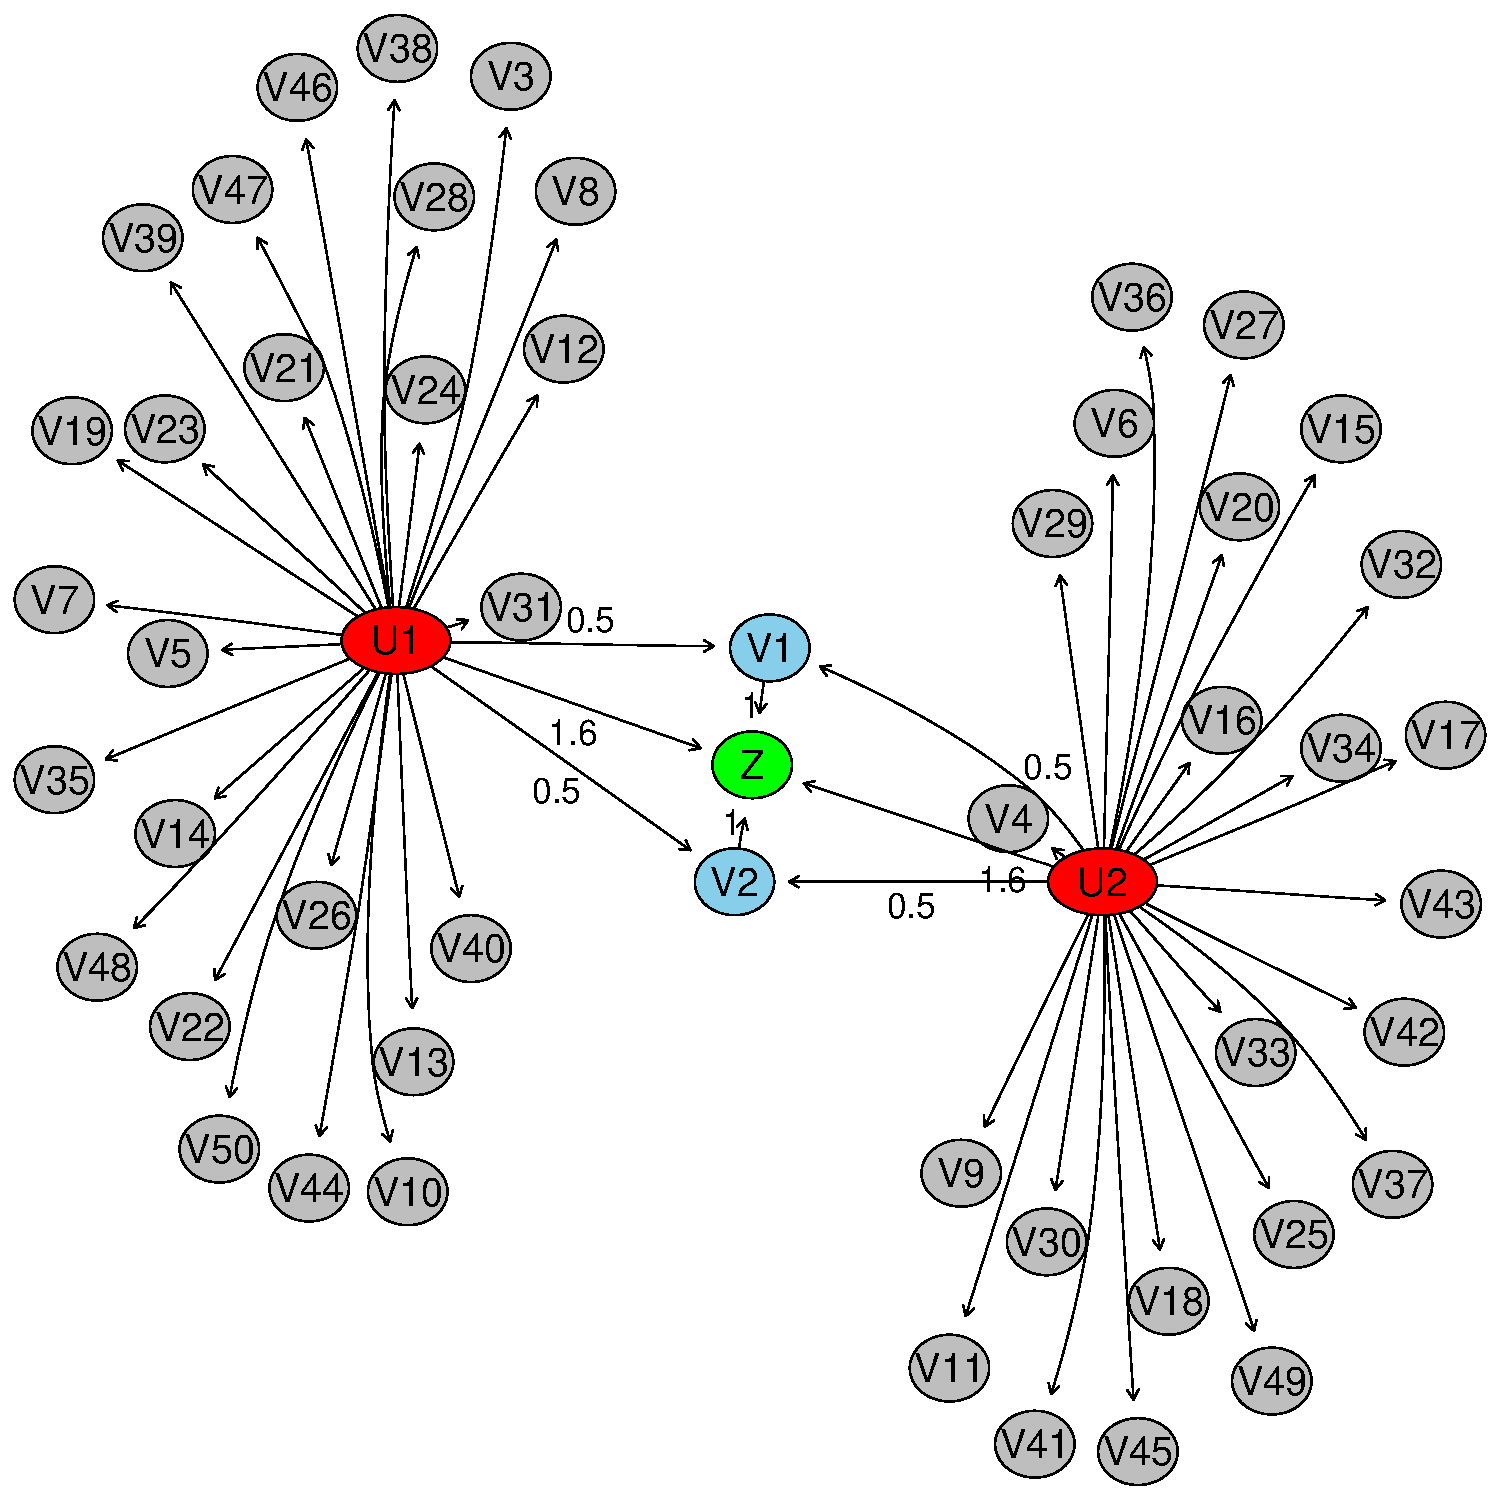
\includegraphics[width=\linewidth]{./images/true_network.pdf}
    \caption{\label{fig_truenet}True network. }
  \end{minipage}\hfill
   \begin{minipage}[t]{0.33\linewidth}
     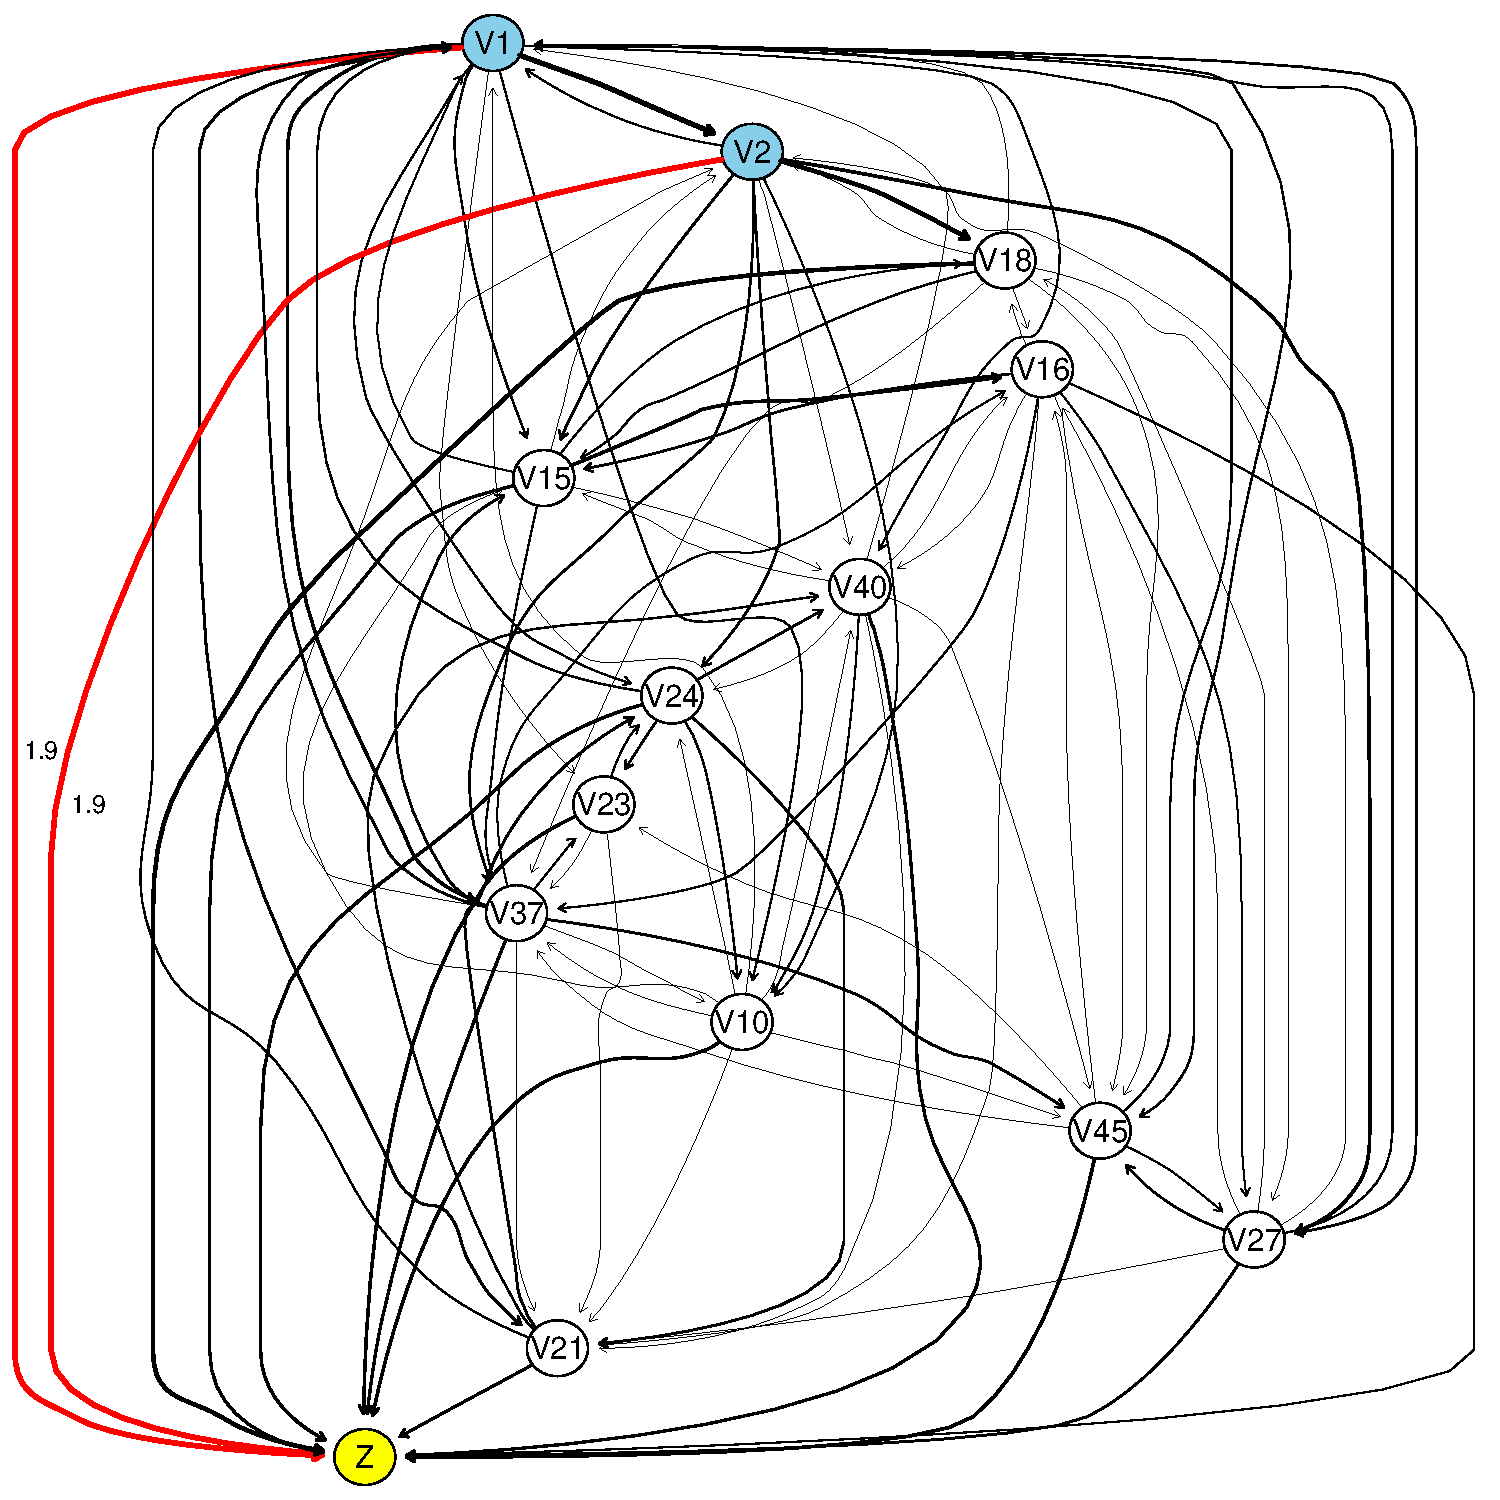
\includegraphics[width=\linewidth]{./images/estimated_network_missingdata.pdf}
     \caption{\label{fig_missing} Estimated network when $U_1$ and
      $U_2$ are unobserved.}
   \end{minipage}\hfill
   \begin{minipage}[t]{0.33\linewidth }
    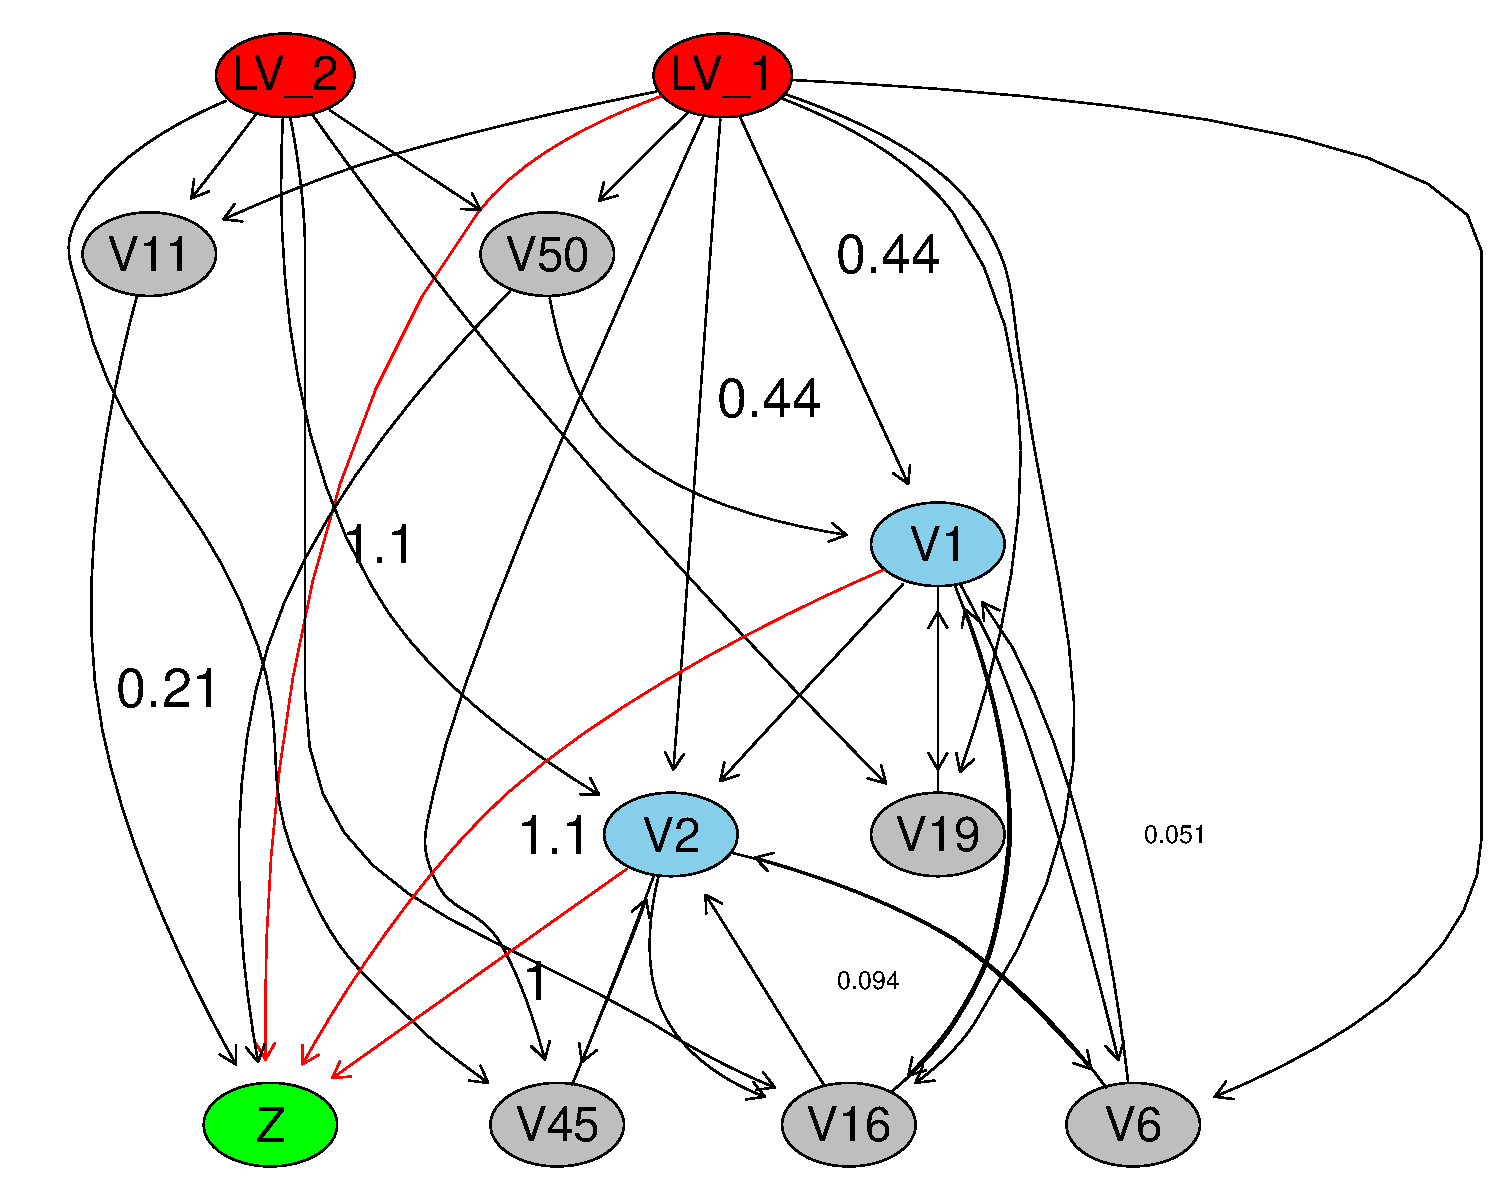
\includegraphics[width=\linewidth]{./images/estimated_network_infered.pdf}
    \caption{\label{fig_estnet_infered} Estimated network at the last
      iteration of algorithm \ref{alg:latentEM}.}
  \end{minipage}
\end{figure}
\begin{figure}[ht]
  \centering
  \begin{minipage}[t]{0.42\linewidth}
    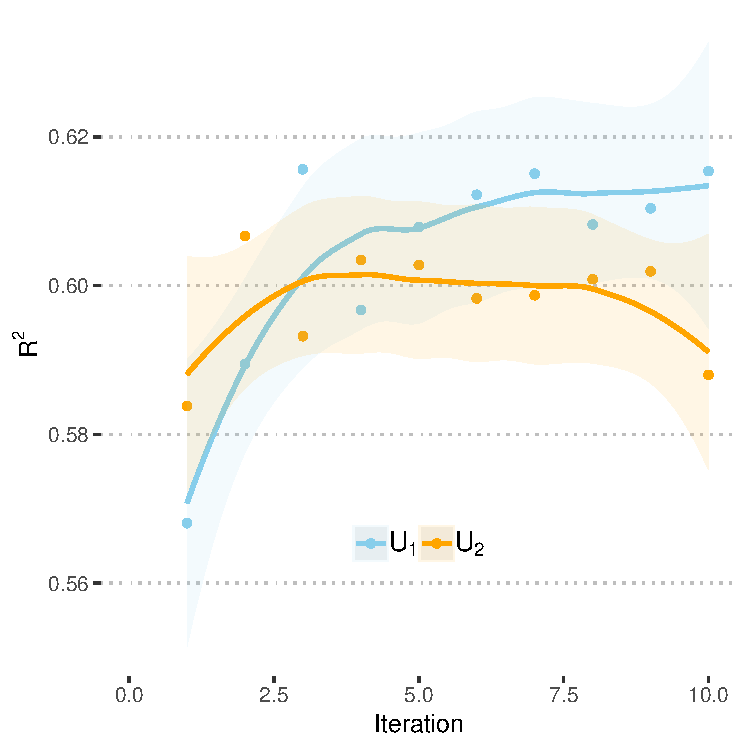
\includegraphics[scale=0.3]{images/fig_paper_r2lat.pdf}
    \caption{\label{fig:latrecons}$R^2$ in the prediction of the latent variable from the selected principal components.\medskip}
  \end{minipage}\hfill
  \begin{minipage}[t]{0.42\linewidth}
    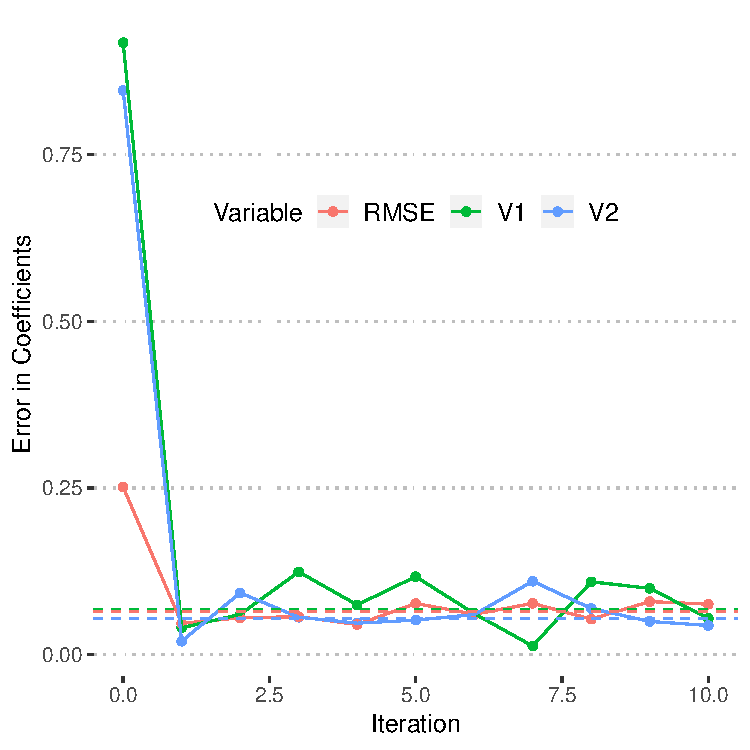
\includegraphics[scale=0.3]{images/fig_paper_errors.pdf}
    \caption{\label{fig:errorcoef}Error in coefficients as a function of the iterations.\medskip}
  \end{minipage}
\end{figure}



\subsection{Experimental Data}
In order to assess the efficacy of our approach on real-world data, we picked a dataset of a type that is typically hard to infer, even with deep learning.  The dataset in question was obtained from the Cure Huntington's Disease Initiative (CHDI) foundation \cite{langfelder_integrated_2016}.  The dataset captured gene expression and CAG repeat expansion of CAG knock-in mice and consisted of striatum gene expression and proteomic data as well as some other miscellaneous measurements.  For the purposes of this analysis, we extracted CAG, weight, mouse age, and a number of gene expression and proteomic measurements, so that gene expression would also have matching proteomic data, and so that top [N - add N] variables rank-correlated with CAG would be present in the analysis.  While the small number of features hampered the inference, the dataset needed to be small enough to be of practical utility for method development.

CAG repeats cause Huntingont's disease via a complex and not entirely understood mechanism, where disease age of onset and severity strongly correlate with repeat length.  Furthermore, CAG influences a large number of gene expression and protein level markers.  Therefore CAG is an ideal pleiotropic covariate of a type that our algorithm should be able to uncover.  In this respect, it's an easy target.  However, in every other respect the dataset is very challenging.  The log-linear range of gene expression and expression/protein level correlations is low; further, though gene expression leads to protein level of a given gene product, this correlation is also often low and is obscured by saturation effects and complex, multi-layered molecular regulation mechanisms.  The sample size is, as mentioned above, quite small.  And finally, though CAG varies across the population, some mice were early knock-ins and were not resequenced, their reported values being the knock-in CAG length, and therefore tied among [M - give the number] animals, making it impossible to infer CAG perfectly in principle.  Assessment of performance was assessed as shown in the table below as well as in the figures.


\begin{figure}[ht!]
  \centering
  \begin{minipage}[t]{0.49\linewidth}
    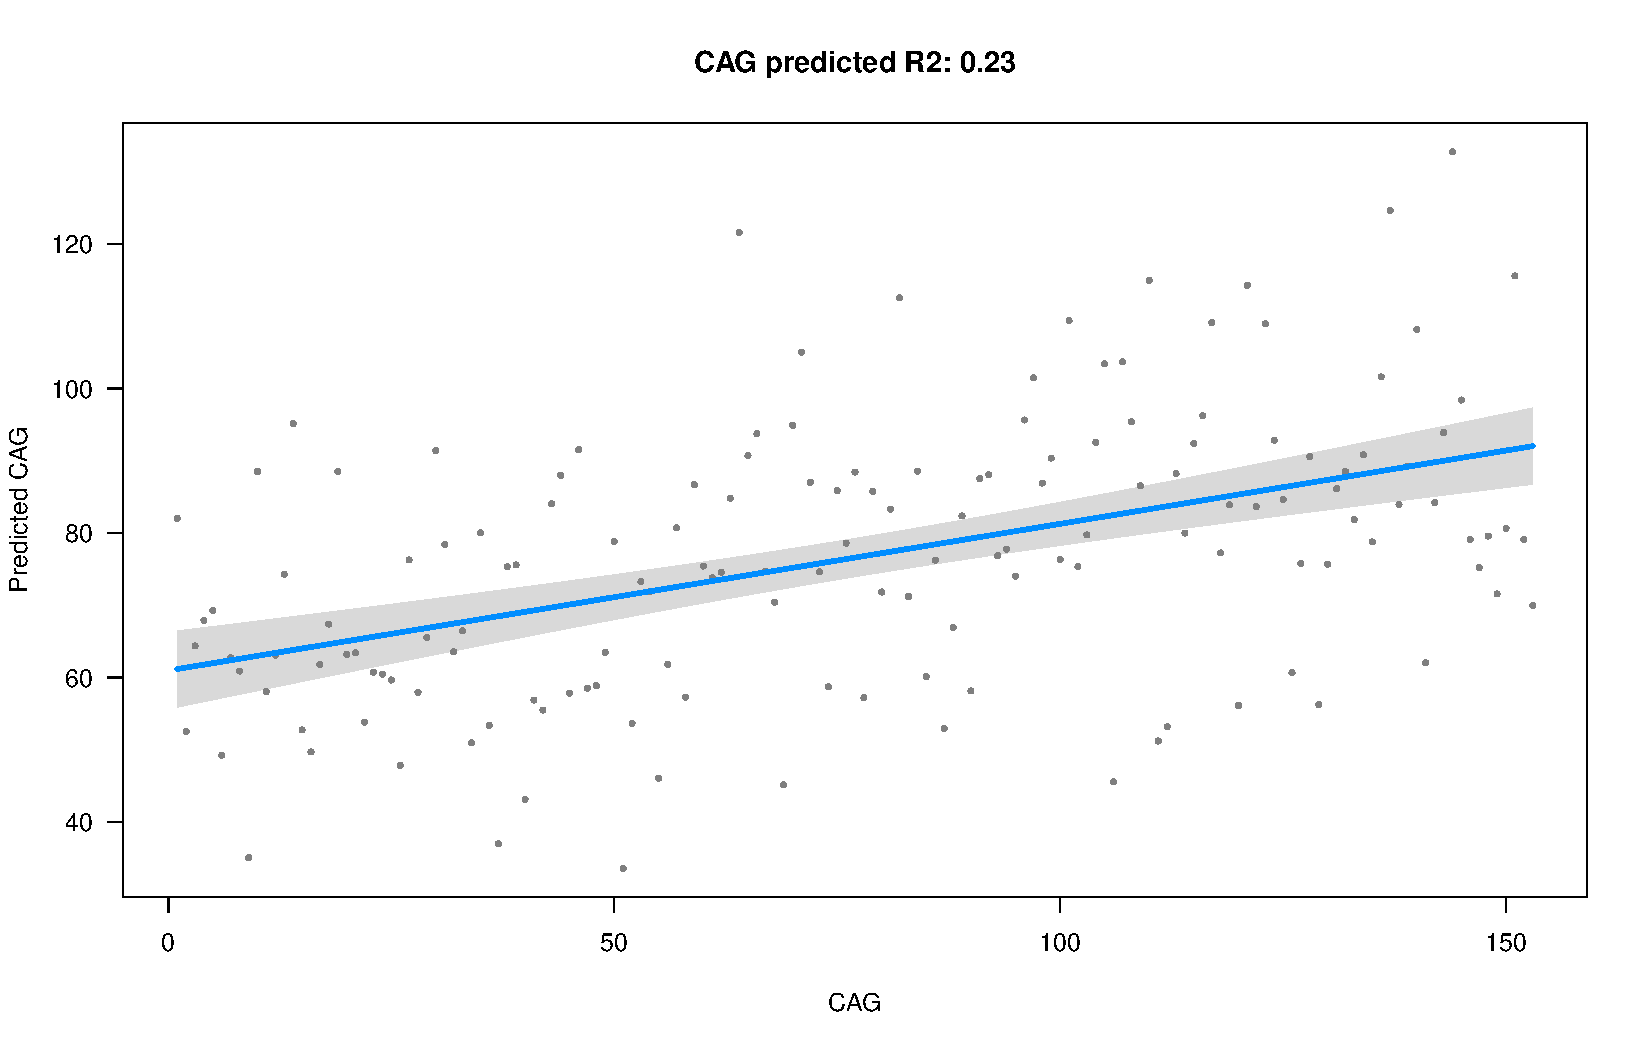
\includegraphics[width=\linewidth]{./images/CAG_linear_boot3_iter10.pdf}
    \caption{\label{fig_cag_linear} Predicted latent variable (CAG) using PCA.}
  \end{minipage}\hfill
   \begin{minipage}[t]{0.49\linewidth}
     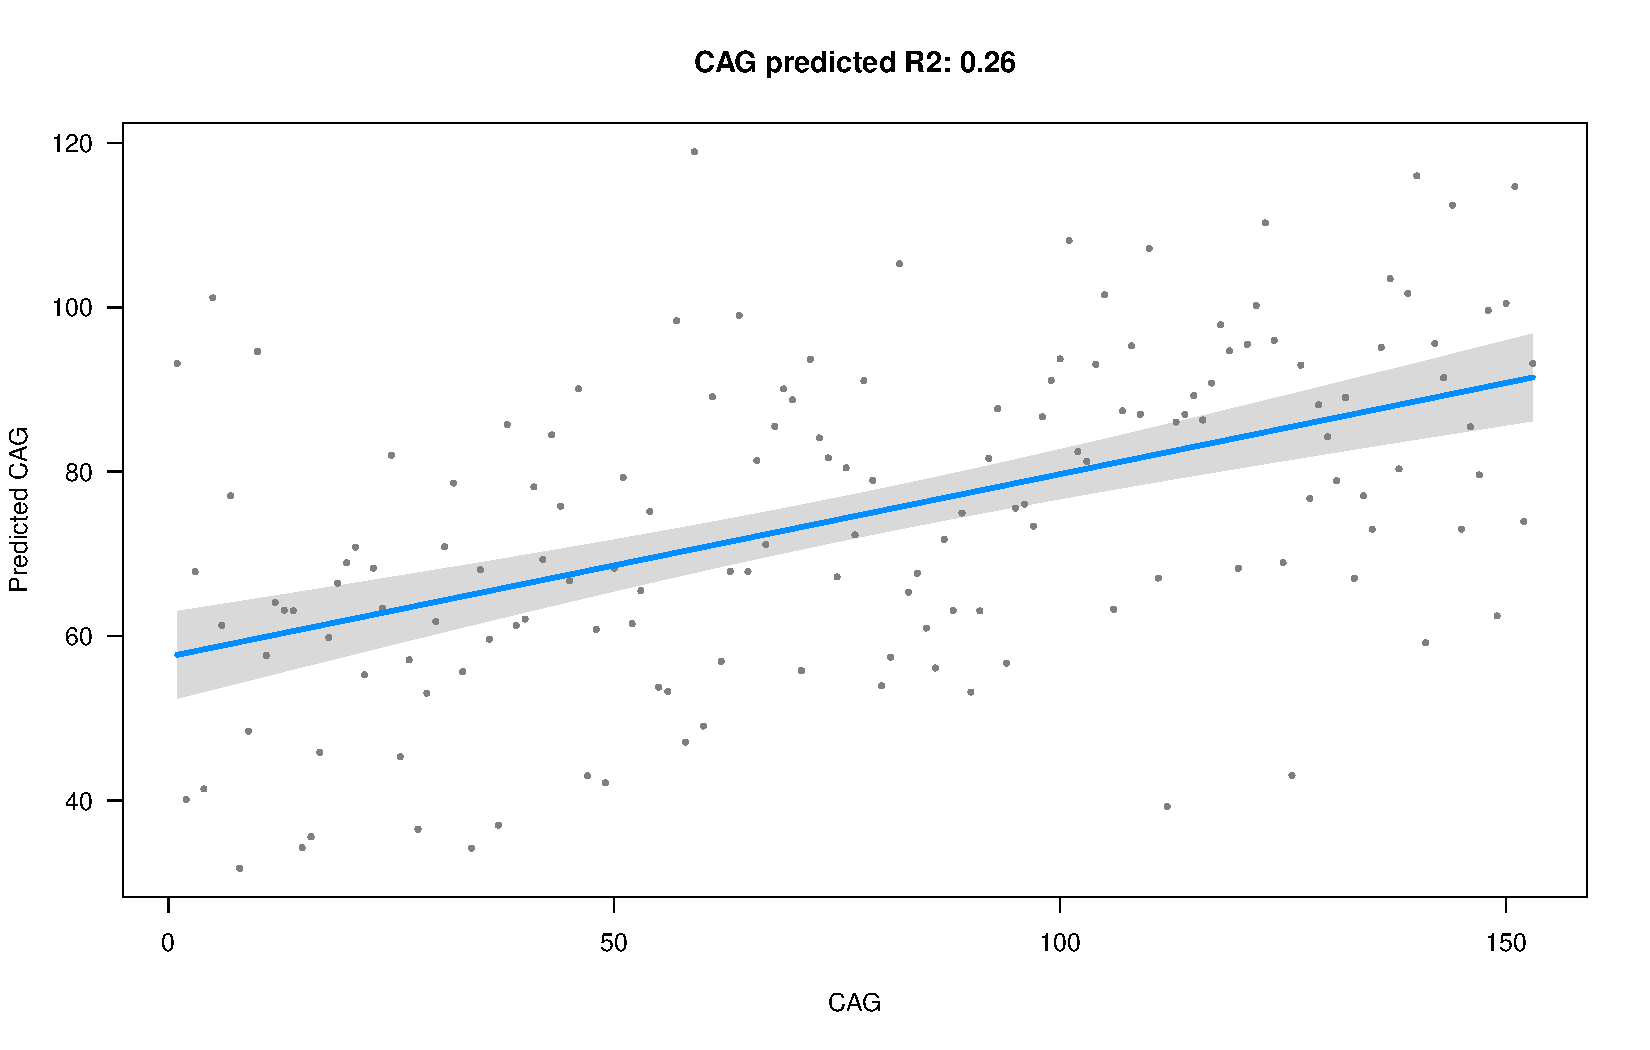
\includegraphics[width=\linewidth]{./images/CAG_autoencoder_boot3_iter10.pdf}
     \caption{\label{fig_cag_ae} Predicted latent variable (CAG) using autoencoder.}
   \end{minipage}\hfill
\end{figure}
\medskip


\begin{algorithm}%[H]
 \caption{Assesment Of Inference Of Latent CAG Repeat Length}
 \label{alg:cag}
\begin{algorithmic}
\STATE {\bfseries Data:} The CAG dataset, with CAG repeat length withheld
\STATE \textbf{Result:} Latent space predictive of CAG in training data and code to predict out of sample
 \STATE Set significance threshold $\alpha$ (e.g. $\alpha = 0.05$)\;
 \STATE Learn $\bar{U} = PCA(R_{\bar{U}})$\;
 \STATE Calculate column-wise variance explained $V_E^{0}$ for $\bar{U}^{*}$\;
 \STATE Set $V_E^s = 0 \times rank(R_{\bar{U}})$, matrix of variances explained by shuffling\;
 \FOR{fold $in$ 5 folds} 
  \STATE Train on 4/5 of the data
  \STATE Learn latent variables using linear and autoencoder approaches
  \STATE Predict out of sample
  \STATE Concatenate all out-of-sample predictions
 \ENDFOR
\STATE Assess $R^{2}$ for linear and autoencoder methods
\end{algorithmic}
\end{algorithm}


\section{Generalizations of this approach}
In this section, we discuss extensions to this approach for GGMs with interactions, nonlinear functional forms, and categorical variables. 

\subsection{Gaussian Graphical Models With Interactions}
In the presence of interactions among variables in a GGM, equation \ref{eq:residualColumn} expressing the deviation of residuals from Gaussian noise may acquire higher-order terms due to interactions among the descendants of the latent space $U$:

\begin{equation}
R_N = \beta_0 + \beta_1 U + \beta_2 U^2 + \beta_2 U^3 + \dots.
\label{eq:residualColumnWithInteractions}
\end{equation}

Assuming interactions up to $k$th power are present in the system being modeled, residuals for each variable may have up to $k$ terms in the model matrix described by equation \ref{eq:residualColumnWithInteractions}, and if interactions among variables in the latent space $U$ also exist, the cardinality of the principal components of the residuals may far exceed the cardinality of the underlying latent space.  Nevertheless, it may be possible to reconstruct a parsimonious basis vector by application of regularization and nonlinear approaches to latent variable modeling, such as nonlinear PCA (e.g. using methods from \cite{karatzoglou_kernlab_2004}), or autoencoders (\cite{louizos_causal_2017}) as will be discussed below.

\subsection{Generalization to nonlinear functions}
We can show that linear PCA will suffice for a set of transformations broader than GGMs without interactions.  In particular, we will focus on nonlinear but homeomorphic functions within the Generalized Additive Model (GAM) family.  When talking about multiple inputs, we will require that the relationship of any output variable to any of the covariates in equation \ref{eq:residualColumn} is homeomorphic (invertible), and that equation \ref{eq:resPCA} can be marginalized with respect to any right-hand-side variable as well as to the original left-hand side variable.  For such class of transformations, mutual information between variables, such as between a single confounder $U$ and some downstream variable $N$, is invariant (\cite{kraskov_estimating_2004}).  Therefore, residuals of any variable $N$ will be rank-correlated to $rank(U)$ in a transformation-invariant way. Further, spearman rank-correlation, specifically, is defined as pearson correlation of ranks, and pearson correlation is a special case of mutual information for bivariate normal distribution.  Therefore when talking about mutual information between ranks of arbitrarily distributed variables, we can use our results for the GGM case above.

Thus, equation \ref{eq:residualColumn} will apply here with some modifications:
\begin{equation}
rank(R_N) = \beta_0 + \beta_1 rank(U) + \xi_N.
\label{eq:residualColumnRank}
\end{equation}

Since a method has been published recently describing how to capture rank-equivalent residuals (aka probability-scale residuals, or PSR) for any ordinal variable (\cite{shepherd_probability-scale_2016}), we can modify the equation \ref{eq:resPCA} to reconstruct latent space up to rank-equivalence when interactions are absent from the network.

\begin{equation}
rank(U) = \frac{1}{\beta_i} rank(R_i) + \frac{1}{\beta_j} rank(R_j) + \dots + \xi. 
\label{resPcaGam}
\end{equation}

When $U$ consists of multiple variables that are independent of each other, the relationship between $N$ and $U$ can be written down using the mutual information chain rule (\cite{mackay_information_2003}) and simplified taking advantage of mutual independence of the latent sources:
\begin{equation}
\label{eq:rankSetRelationship}
\begin{split}
I(N; U) = I(N; U_1, U_2, \dots, U_U) \\= \sum_{i=1}^{u}{I(N; X_i | X_{i-1}, \dots, X_1)} = \sum_{i=1}^{u}{I(N; X_i)}.
\end{split}
\end{equation}

If interactions among $U$ are present, it may still be possible to approximate the latent space with a suitably regularized nonlinear basis, but we do not, at present, know of specific conditions when this may or may not work.  Novel methods for encoding basis sets, such as nonlinear PCA (implemented in the accompanying code), autoencoders, and others, may be brought to bear to collapse the linearly independent basis down to non-linearly independent (i.e. in the mutual information sense) components.

While approximate inference of latent variables for GMs built over invertible functions had been noted in \cite{elidan_ideal_2007}, the above method gives a direct rank-linear approach leveraging the recently-proposed PSRs.

\subsection{Generalization to categorical variables}
In principle, PSRs can be extended to the case of non-ordinal categorical variables by modeling binary in/out of class label, deviance being correct/false.  These models would lack the smooth gradient allowed by ranks and would probably converge far worse and offer more local minima for EM to get stuck in.  

\section{Conclusions and Future Directions}
In this work we present a method for describing the latent variable space that is optimal under linearity, up to rank-linearity.  When we cannot provide such guarantees, the method will still identify the terms of the model matrix of the latent space, including any interactions, for models in the GGM family, making it possible to attempt to infer the original (compact) latent space by non-linear modeling and regularization.  The method does not place \textit{a priori} constraints on the number of latent variables, and will infer the upper bound on this dimensionality automatically.  This method is a generalization of prior work, both in terms of the global treatment of the residual space, and in terms of stronger statements of applicability in cases when probability-scale residuals are applicable.  

To address cases where the internal wiring of the latent case is unimportant and the confounding may be non-linear, we provide an autoencoder implementation to supplement our PCA and rank-PCA approaches.  In this case, we use linear PCA (\ref{alg:linearPCA}) to set the cardinality of the bottleneck layer of the autoencoder.  Using autoencoders has been shown to be of high utility when the structure of the causal model is already known (\cite{louizos_causal_2017}).  Learning structure over observed data as well as unconstrained latent space via autoencoders, as in our work, result in a hybrid "deep causal" model that would be useful, for instance, in epidemiological problems, when, in general, neither the model structure, nor the latent space are well-understood \textit{a priori}.  In epidemiological applications, it is highly desirable to retain original features of the data for explainability but is also helpful to introduce latent variables to account for unobserved (pleiotropic) confounding.  As noted above, calculation of ACE in epidemiological problems is one specific use case.  Applications of such "deep causal networks" should also arise outside of the realm of epidemiology, the traditional causal domain.  For instance, in computer vision coupled with sensor data, or in the nascent internet-of-things paradigm, retention of some features explicitly coupled with the discovery of latent compressed structure may enable inference of cause-and-effect and robust learning, resulting in structures simpler than those generated by multi-layer deep networks.

\clearpage
% \section*{Acknowledgments}
% The authors gratefully acknowledge Karl Runge of GNS Healthcare for his invaluable feedback and suggestions.
 
\small
\bibliography{LatentVars}
\bibliographystyle{icml2020}

\end{document}
